\apendice{Plan de Proyecto Software}\label{anex:A}

\section{Introducción}

%Ref david goo bees https://github.com/davidmigloz/go-bees puede ayudar con la memoria
Una de las primeras actividades de un proyecto software es la planificación. En esta fase se estima el tiempo, esfuerzo y dinero que se espera invertir en el proyecto. El objetivo principal de la fase de planificación es estimar si se puede realizar el proyecto con éxito y, en ese caso, tener una guía de referencia para el proceso de desarrollo. Este anexo recoge los documentos generados en este proceso y se divide en dos partes:
\begin{description}
	\tightlist
	\item[Planificación temporal.] En esta parte se estima el tiempo y el esfuerzo que se requieren para la realización del proyecto.
	\item[Estudio de la viabilidad.] Esta parte se estima si el proyecto es viable tanto económica como legalmente, por tanto se dividirá en dos secciones:
	\begin{description}
		\tightlist
		\item[Viabilidad económica.] Análisis del coste y del beneficio que supondría la realización del proyecto en un entorno laboral real.
		\item[Viabilidad legal.] Análisis de las leyes que se aplicarían desde el comienzo del proyecto. En un proyecto software tienen especial importancia las licencias y la Ley de Protección de Datos.
	\end{description}
\end{description}

\section{Planificación temporal}

La planificación temporal del proyecto ha tomado como referencia el modelo de ciclo de vida \textbf{SCRUM} \cite{scrum_master_scrum_2019}:
\begin{itemize}
	\item Se ha aplicado un desarrollo incremental y evolutivo.
	\item Se han realizado iteraciones (\textit{sprints}) de dos semanas. Se finalizaba el sprint con una reunión entre el tutor y el alumno que daba comienzo al siguiente sprint y que constaba de dos partes:
	\begin{itemize}
		\item Una parte de revisión del sprint en la que se exponía una parte operativa del producto realizada durante el sprint.
		\item Otra de planificación del siguiente sprint en la que se determinaba el trabajo y los objetivos a alcanzar durante el siguiente sprint. Esto quedaba reflejado como una pila de tareas que se debían completar durante el sprint y que han sido registradas en el sistema de gestión de incidencias de GitLab.
	\end{itemize}
\end{itemize}

\subsection{Sprints}

Aún habiendo seguido un proceso incremental, según la naturaleza de los sprints y el orden en el que se han llevado a cabo, en el proceso del desarrollo se pueden diferenciar varias etapas:
\begin{itemize}
	\item  Una primera etapa de \textbf{investigación} de las herramientas que se utilizarán durante el proceso y de \textbf{configuración} del entorno de desarrollo.
	
	\item En la segunda etapa se aprecian tareas de \textbf{diseño e implementación} de la parte lógica de la aplicación. Se diseña el framework de conexión a forjas de repositorios, se implementa el framework descrito en \textit{Soporte de Métricas con Independencia del Lenguaje para la Inferencia de Refactorizaciones} \citep{marticorena_sanchez_soporte_2005} para el cálculo de métricas y se diseñan los modelos de datos que serán utilizados por la aplicación.
	
	\item Durante la segunda etapa se apreció que se debía mejorar el flujo de trabajo con herramientas de automatización de actividades como pruebas, despliegue, revisión de calidad, etc.
	
	\item Etapa  de diseño e implementación de la \textbf{interfaz gráfica} y \textbf{mejora de funcionalidades}.
	
	\item Etapa de \textbf{documentación} en la que se escribe la memoria y los anexos. También se preparan videotutoriales y manuales de usuario.
\end{itemize}

A continuación se describe cada una de las etapas del proyecto y sus respectivas actividades. Se acompañará la descripción con capturas de pantalla tomadas del repositorio del proyecto en GitLab \footnote{Enlace al repositorio del proyecto: \url{https://gitlab.com/mlb0029/comparador-de-metricas-de-evolucion-en-repositorios-software}} y de \textit{gráficos burndown} de los \textit{milestones} asociados a cada uno de los sprints del ciclo de vida del proyecto.

\subsubsection{Investigación y configuración}

La etapa de investigación y configuración comenzó a principios de octubre y duró \textbf{3 sprints} (6 semanas) y sus decisiones afectaron a todo el proyecto. Se recopiló información sobre trabajos relacionados como \textit{Activiti-Api} \cite{blanco_alonso_activiti-api_2016}, \textit{Soporte de Métricas con Independencia del Lenguaje para la Inferencia de Refactorizaciones}  \cite{marticorena_sanchez_soporte_2005} y \textit{sPACE: Software Project Assessment in the Course of Evolution} \cite{ratzinger_space:_2007}, y se estudió los entornos y herramientas que se utilizarían para el desarrollo del proyecto.

En la Fig. \ref{fig:AnexA_S_1} se pueden apreciar los milestones definidos durante esta etapa, su descripción, la fecha de apertura y cierre, y el número de issues asociadas. La mayoría de issues asociados a estos milestones están etiquetadas como `\textit{Research}' (Estudio o investigación) y `\textit{Project Configuration}' (Configuración del proyecto).

\begin{figure}[!h]
	\centering
	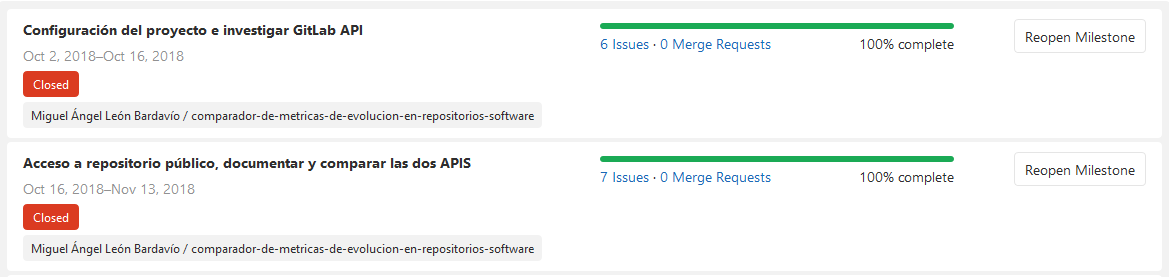
\includegraphics[scale=0.40]{AnexA_S_1}
	\caption{Milestones asociados a la etapa de investigación y configuración}
	\label{fig:AnexA_S_1}
\end{figure}
\FloatBarrier

Del primer milestone no se ha podido sacar un gráfico burndown, debido a problemas con GitLab. Sin embargo, se muestra gráfico burndown del segundo milestone en la Fig. \ref{fig:AnexA_Bd_1}.

\begin{figure}[!h]
	\centering
	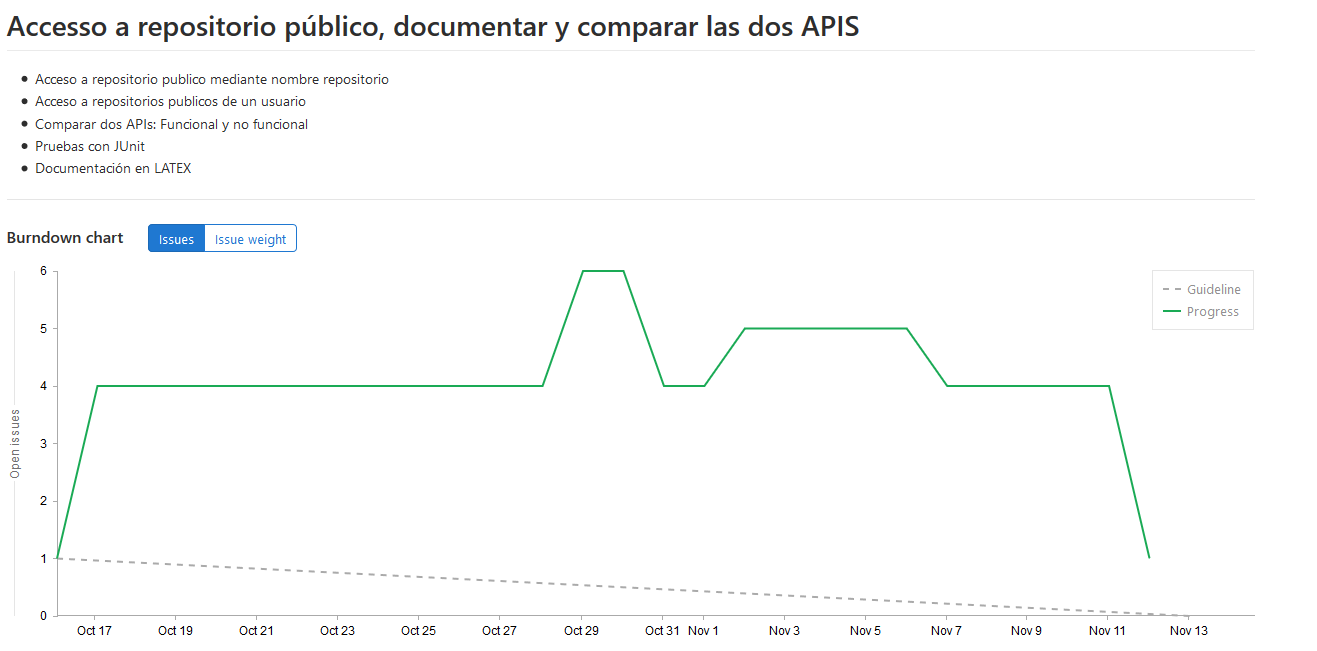
\includegraphics[scale=0.40]{AnexA_Bd_1}
	\caption{Gráfico burndown del segundo sprint Acceso a repositorio público, documentar y comparar las dos APIS}
	\label{fig:AnexA_Bd_1}
\end{figure}
\FloatBarrier

\subsubsection{Diseño e implementación}

Después de esta etapa de investigación, comenzó una etapa de diseño. Las tareas que se definen se relacionan con el diseño de la parte lógica del sistema software a construir. Esta etapa de diseño tuvo duración de \textbf{5 sprints} y se dedicó un sprint adicional para la configuración del flujo de trabajo que se explica en el siguiente apartado.

\begin{figure}[!h]
	\centering
	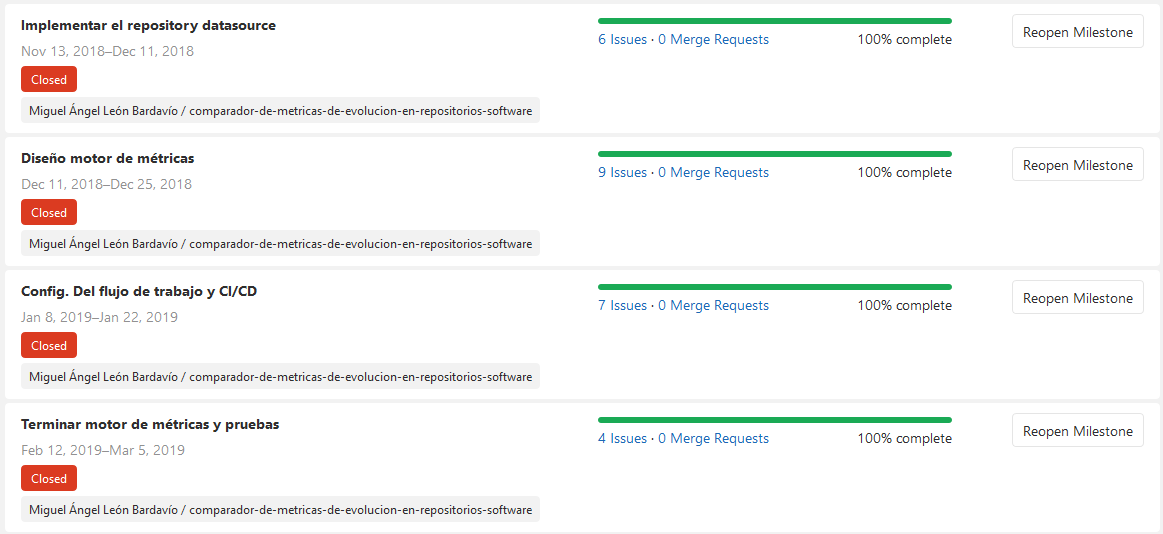
\includegraphics[scale=0.40]{AnexA_S_2Y3}
	\caption{Sprints de la etapa de diseño e implementación y de la etapa de configuración del flujo de trabajo}
	\label{fig:AnexA_S_2Y3}
\end{figure}
\FloatBarrier

En la Fig. \ref{fig:AnexA_S_2Y3} se muestran 3 milestones asociados a esta etapa y otro asociado a la etapa siguiente, que pausó la etapa de diseño durante un sprint.
Los milestones asociados a la etapa de diseño son:
\begin{itemize}
	\item \textbf{\textit{Implementar el repository datasource}} (2 sprints). Consta de una tarea (\href{https://gitlab.com/mlb0029/comparador-de-metricas-de-evolucion-en-repositorios-software/issues/22}{\#22}) etiquetada como `\textit{Design}' para implementar el framework de conexión a GitLab y obtener la información de los repositorios. El resto de tareas están mal definidas, se han etiquetado como `\textit{Future}' (Para hacer en el futuro) o `\textit{Badly Defined}' (Mal definidas) y se definieron en los milestones posteriores.
	
	\item \textbf{\textit{Diseño motor de métricas}} (1 sprint). Todas las tareas en este milestone se han definido con label `\textit{Design}' (Diseño). Es destacable el gráfico burndown de este milestone, como se puede observar en el segundo gráfico de la Fig. \ref{fig:AnexA_Bd_2Y3}.
	
	\item \textbf{\textit{Terminar motor de métricas y pruebas}} (2 sprints). Consta de cuatro issues: 3 de aumento de características (etiqueta `\textit{Feature}') y una de pruebas (etiqueta `\textit{Test}').
\end{itemize}

En la Fig. \ref{fig:AnexA_Bd_2Y3} se muestran los gráficos burndown de los dos primeros milestones de esta etapa. No se puedo obtener el gráfico del tercer milestone.

\begin{figure}[!h]
	\centering
	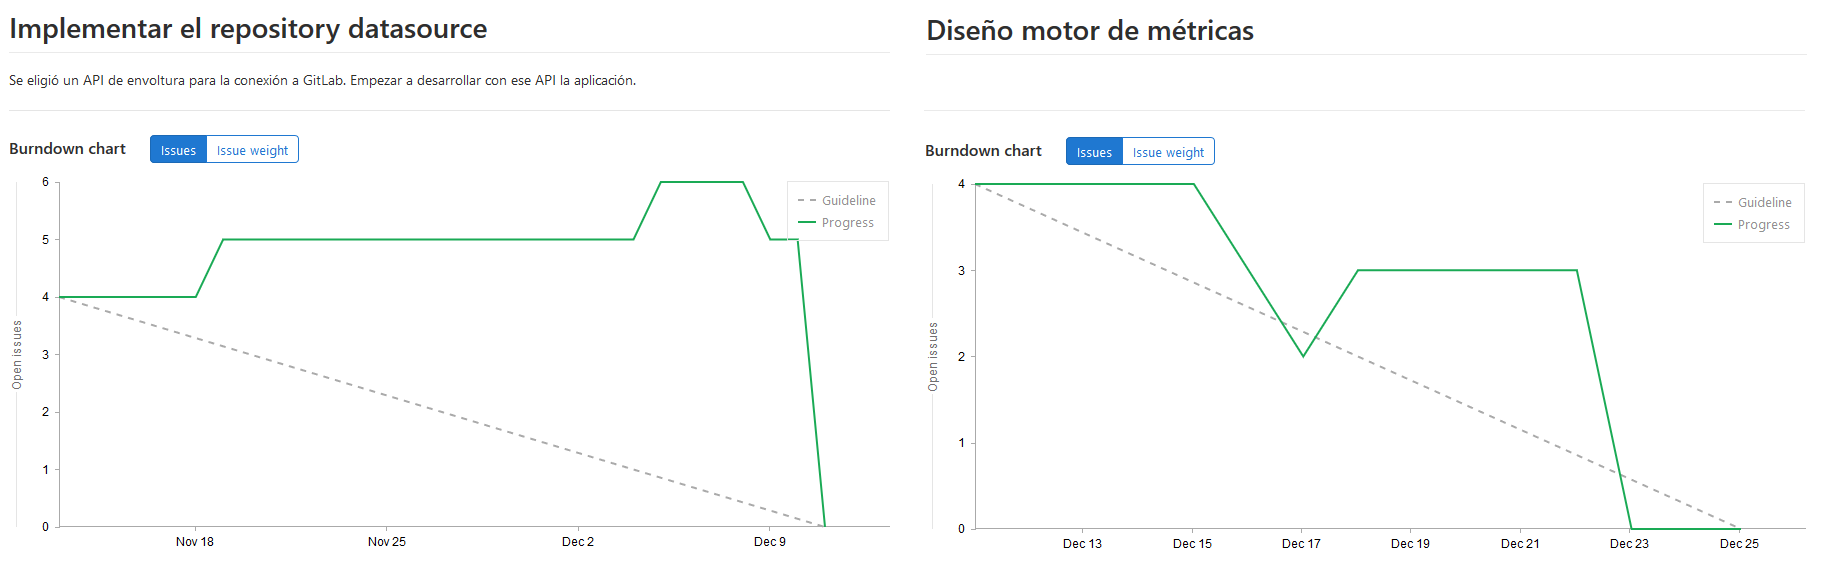
\includegraphics[scale=0.27]{AnexA_Bd_2Y3}
	\caption{Gráficos burndown de }
	\label{fig:AnexA_Bd_2Y3}
\end{figure}
\FloatBarrier

El primero muestra la evolución del primer milestone (\textit{Implementar el repository datasource}). Se aprecia la definición incorrecta de issues a mitad del sprint, que se cerraron al final del milestone marcándolas como `\textit{Future}' o `\textit{Badly Defined}'.

En el segundo gráfico se muestra la evolución del segundo milestone (\textit{Diseño motor de métricas}). La evolución fue bastante buena, completando las tareas antes de tiempo. Se observa que se definió una issue (\href{https://gitlab.com/mlb0029/comparador-de-metricas-de-evolucion-en-repositorios-software/issues/30}{\#30}) en mitad del sprint. Dicha tarea se marcó con la etiqueta `Question' y fue para preguntar dudas al tutor. Es destacable la evolución de esa tarea, siendo posible apreciarla a partir de los comentarios realizados en la misma.

\subsubsection{Configuración del flujo de trabajo}

Dentro de la fase de diseño se decidió dedicar \textbf{un sprint} a configurar el proyecto para facilitar el flujo de trabajo y las reuniones de revisión/planificación del sprint. Las principales tareas para mejorar el flujo de trabajo fueron:
\begin{itemize}
	\item Configurar la gestión del proyecto con Maven
	\item Configurar los procesos de integración y despliegue continuo con GitLab (CI/CD)
	\item Realizar pruebas unitarias con JUnit y automatizar su ejecución gracias a Maven y los \textit{pipelines} (CI/CD) de GitLab .
	\item Configurar revisiones automáticas de calidad y de cobertura de las pruebas gracias a Codacy, Jacoco y GitLab.
	\item Configurar un entorno en Heroku donde poder desplegar la aplicación y así poder ser revisada por el tutor fácilmente.
	\item Configurar badges \footnote{Son placas que aportan información rápida sobre el estado del proyecto en ciertos aspectos como la cobertura, la calidad de código o el estado del proceso de CI/CD} para representar los el estado de la calidad de código, cobertura, despliegue y los trabajos de CI/CD.
\end{itemize}

En la Fig. \ref{fig:AnexA_S_2Y3} se muestra este sprint en el milestone llamado `\textit{Config. Del flujo de trabajo y CI/CD}'. Consta de 7 tareas de configuración, pregunta e investigación junto con un par de tareas de test. No se ha obtenido el gráfico burndown de este milestone.

\subsubsection{Implementación de la interfaz gráfica y mejora de las características}

Es la etapa más extensa, duró 14 semanas (\textbf{7 sprints}) y se destacan las etiquetas `GUI' y `Feature'. 

La etapa comienza con un estudio de la herramienta Vaadin para crear la interfaz gráfica y la viabilidad de su uso en el proyecto. Para ello, se realizaron varias pruebas de integración con el entorno de desarrollo (Versión de Java, Eclipse, Maven, etc), se realizó un primer prototipo sencillo y se comprobó que se podría hacer una interfaz gráfica con la licencia gratuita. Una vez terminado con éxito estas pruebas de viabilidad, comenzó el desarrollo de la interfaz gráfica del proyecto.

La interfaz gráfica da un aspecto más visible de lo que el proyecto podría llegar a ser. Los requisitos funcionales evolucionaban conforme evolucionaba la interfaz. Por ejemplo, se decidió agregar varias formas de añadir un repositorio y añadir más formas de conectarse a GitLab.


Se han definido 9 milestones, cometiendo el error de definir varios milestones a la vez para separar la naturaleza de las issues. En la Fig. \ref{fig:AnexA_S_4} se aprecia la descripción, tiempo y número de issues asociadas a cada milestone.

\begin{figure}[!h]
	\centering
	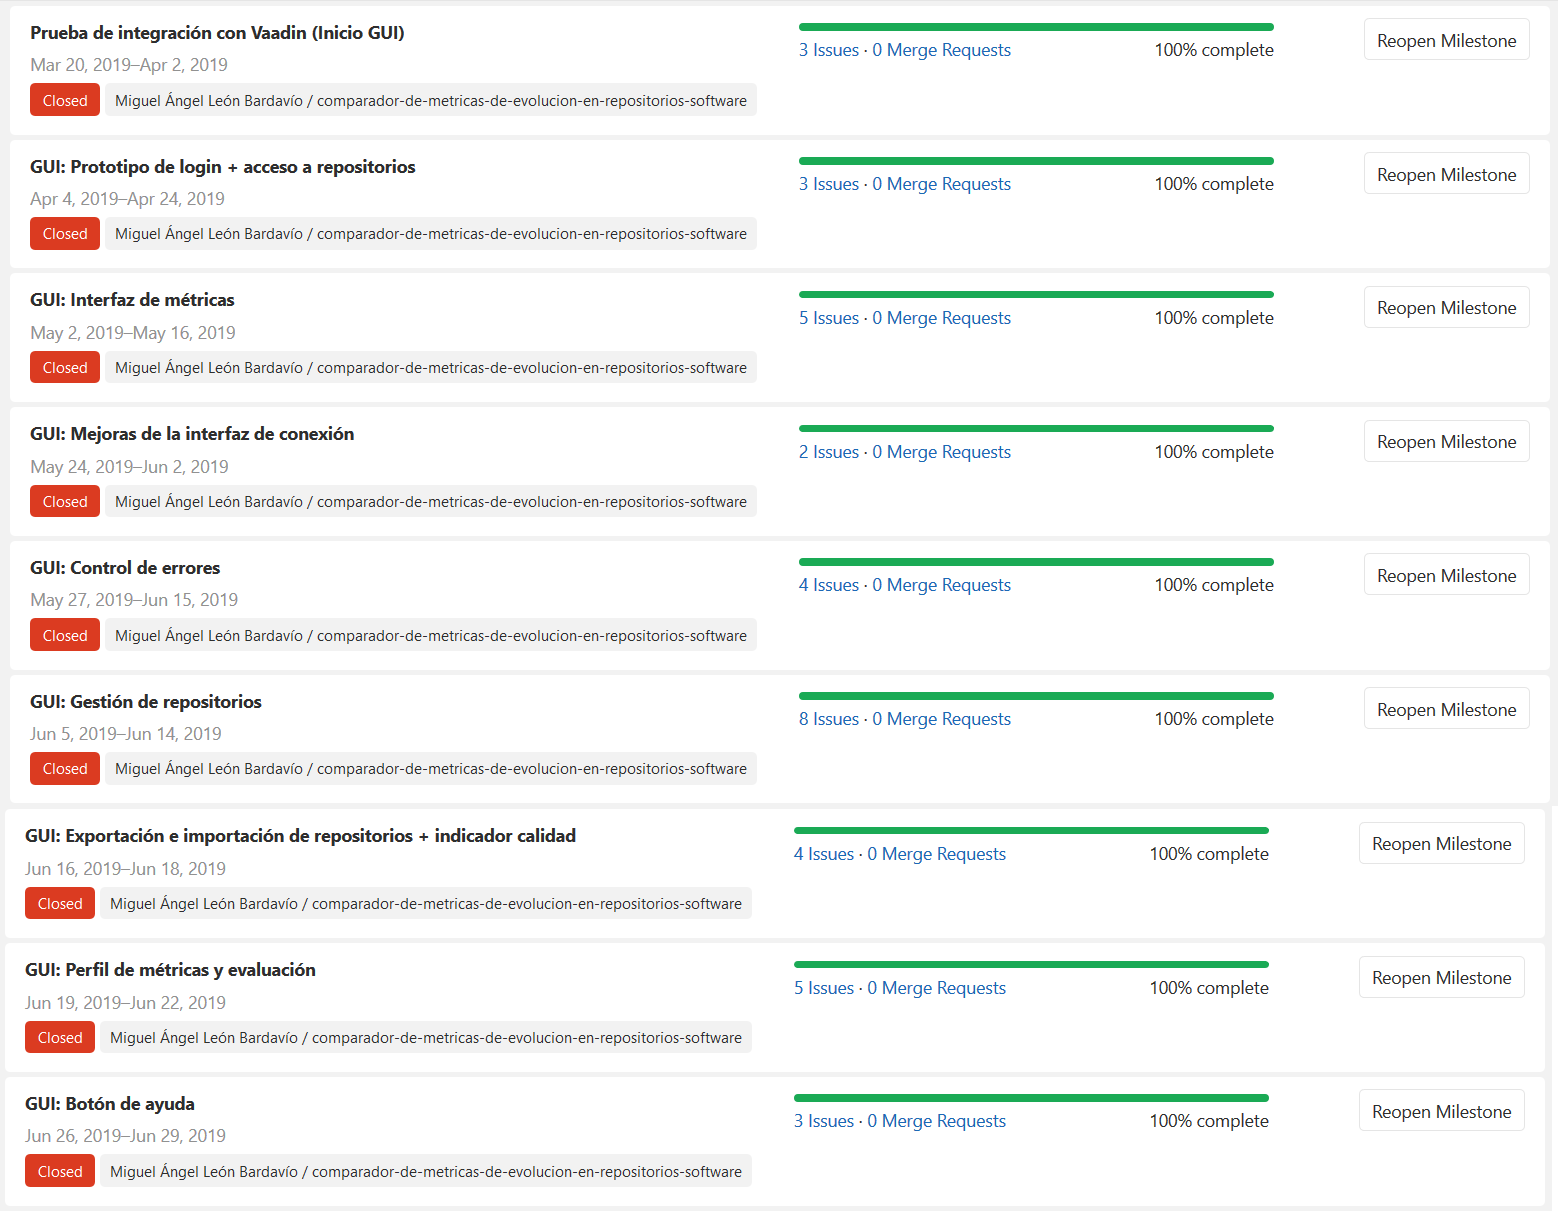
\includegraphics[scale=0.27]{AnexA_S_4}
	\caption{Milestones de la etapa de implementación de la interfaz gráfica y mejora de las características}
	\label{fig:AnexA_S_4}
\end{figure}
\FloatBarrier

Algunos de los gráficos burndown más destacables de esta etapa se muestran en la Fig. \ref{fig:AnexA_Bd_4}

\begin{figure}[!h]
	\centering
	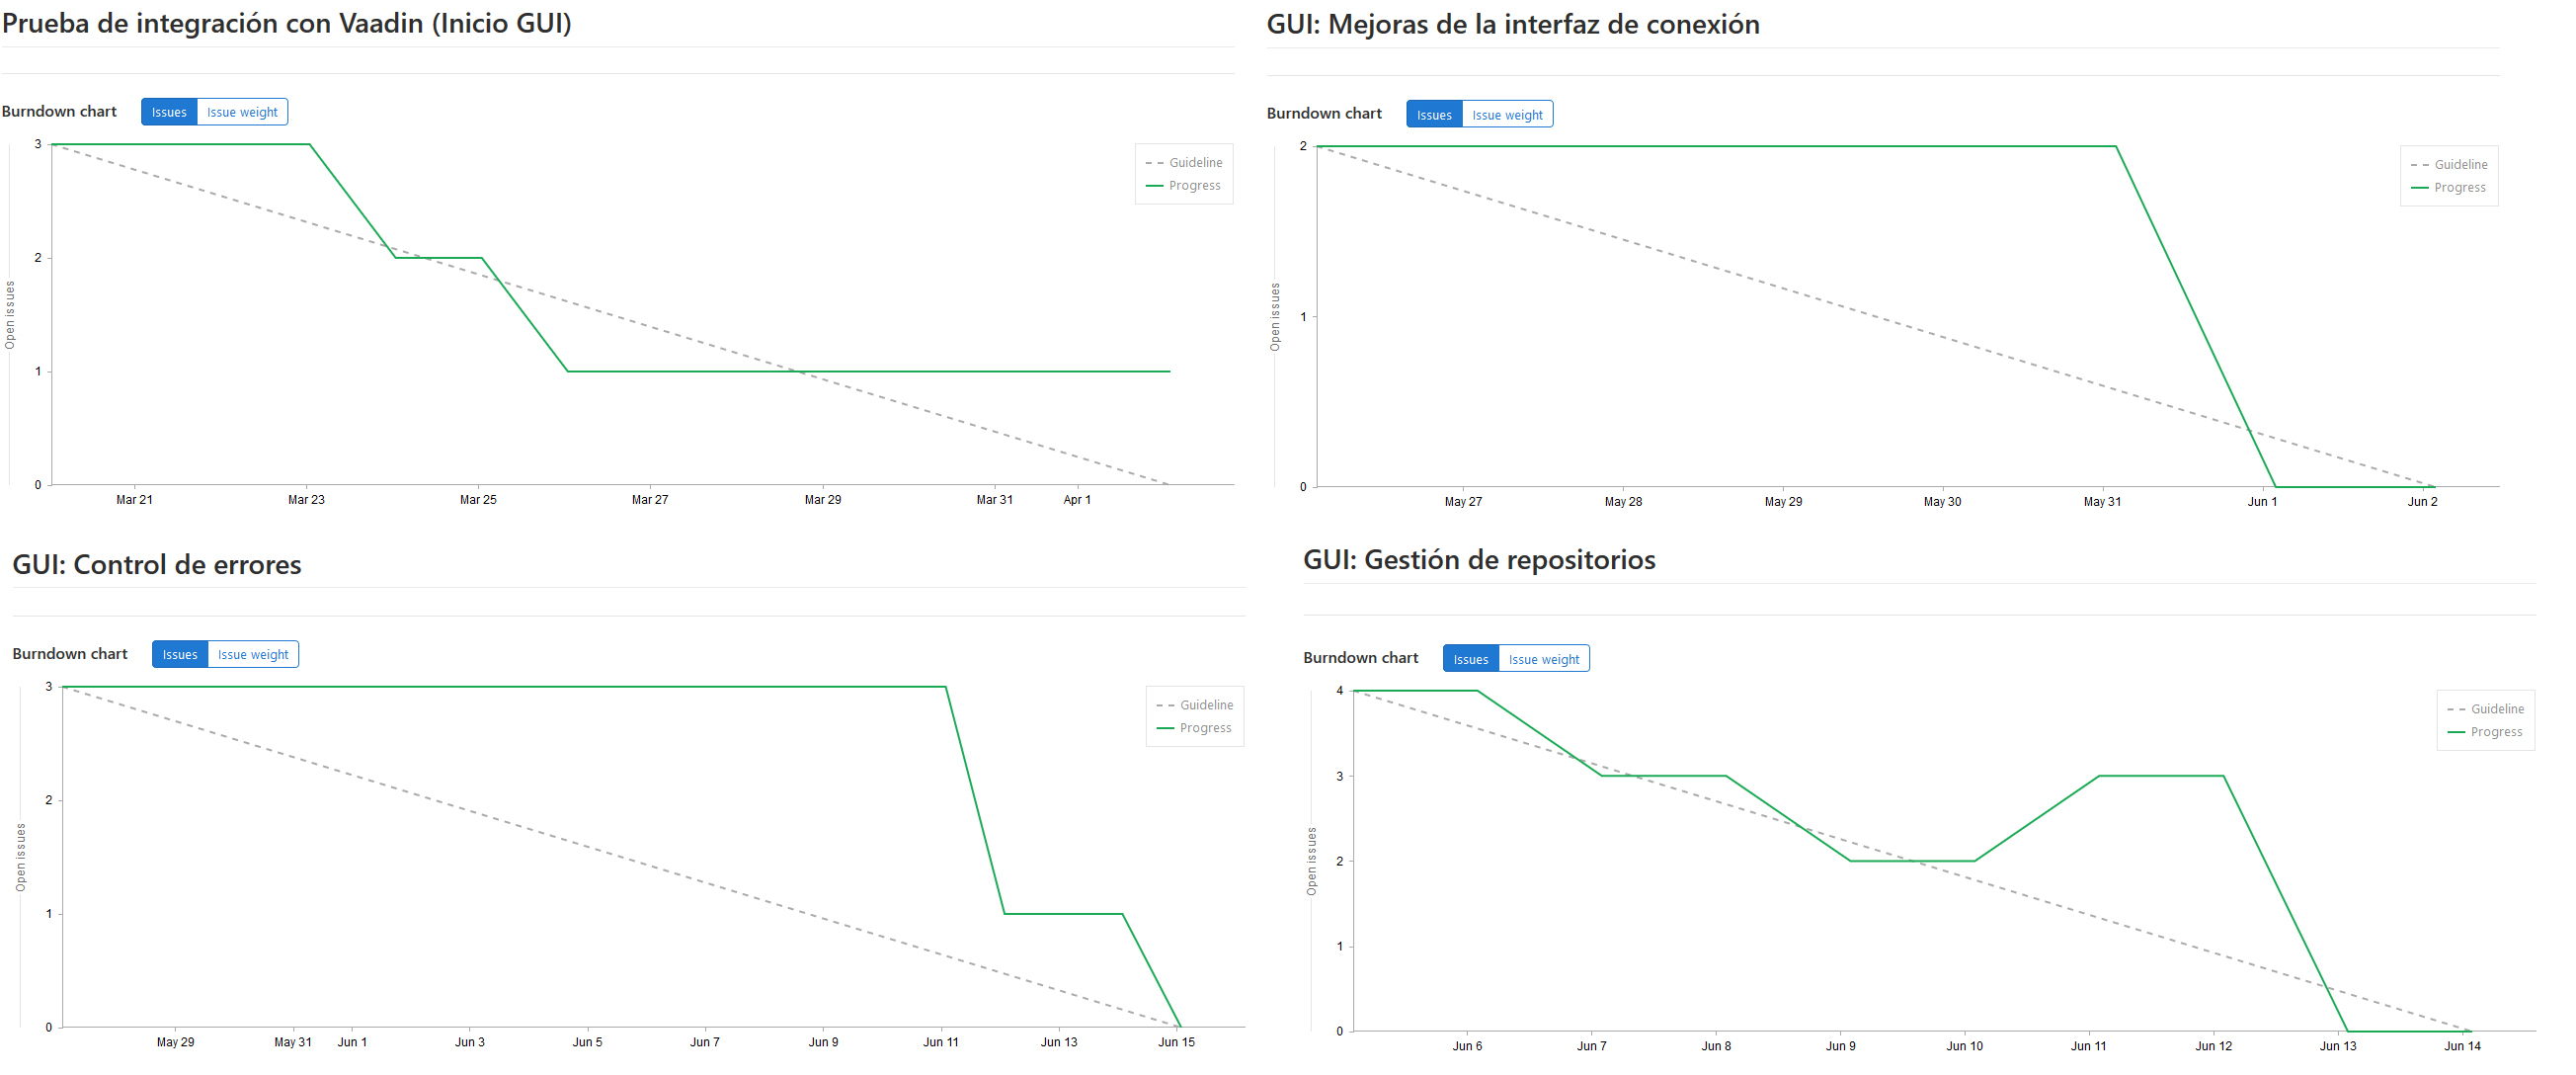
\includegraphics[scale=0.27]{AnexA_Bd_4}
	\caption{Milestones de la etapa de implementación de la interfaz gráfica y mejora de las características}
	\label{fig:AnexA_Bd_4}
\end{figure}
\FloatBarrier

\subsubsection{Documentación}
Esta etapa comenzó al terminar el desarrollo de la aplicación. En esta se realiza la memoria y los anexos del proyecto, así como videotutoriales u otros manuales de usuario. Esta fase tiene una duración aproximada de \textbf{5 sprints}. Se tiene la aproximación debido a que se fue trabajando sin crear su milestone correspondiente. Actualmente se ha creado uno que define las actividades a realizar, pero no describe el tiempo invertido.

\section{Estudio de viabilidad}
\subsection{Viabilidad económica}
En esta sección se realiza un análisis coste-beneficio del proyecto de haberse realizado en un entorno laboral real.

\subsubsection{Costes}
\textbf{Costes de personal}

El proyecto ha sido realizado por un empleado a media jornada (20 horas semanales) durante 11 meses (octubre 2018 --- septiembre 2019). Se considera:
\begin{itemize}
	\tightlist
	\item Salario neto mensual: 600 \officialeuro
	\item Una retención del IRPF por actividad profesional con carácter general del 15\% \cite{agencia_tributaria_cuadro_2019}
	\item Una retribución a la Seguridad Social de 29,9\% \cite{ministerio_de_empleo_y_seguridad_social_bases_2019}: Contingencias comunes (23,6\%) +  Desempleo de tipo general (5,5\%) +  FOGASA (0,20\%) + Formación profesional (0,6\%)
\end{itemize}

Realizando cálculos, se obtiene:
\begin{longtable}[]{@{}lr@{}}
	\toprule
	\begin{minipage}[b]{0.38\columnwidth}\raggedright\strut
		\textbf{Concepto}\strut
	\end{minipage} & \begin{minipage}[b]{0.20\columnwidth}\raggedright\strut
		\textbf{Coste}\strut
	\end{minipage}\tabularnewline
	\midrule
	\endhead
	\begin{minipage}[t]{0.38\columnwidth}\raggedright\strut
		Salario mensual neto\strut
	\end{minipage} & \begin{minipage}[t]{0.20\columnwidth}\raggedright\strut
		600 \officialeuro\strut
	\end{minipage}\tabularnewline
	\begin{minipage}[t]{0.38\columnwidth}\raggedright\strut
		Retención IRPF (15\%)\strut
	\end{minipage} & \begin{minipage}[t]{0.20\columnwidth}\raggedright\strut
		163,34 \officialeuro\strut
	\end{minipage}\tabularnewline
	\begin{minipage}[t]{0.38\columnwidth}\raggedright\strut
		Seguridad Social (29,9\%)\strut
	\end{minipage} & \begin{minipage}[t]{0.20\columnwidth}\raggedright\strut
		325,59 \officialeuro\strut
	\end{minipage}\tabularnewline
	\begin{minipage}[t]{0.38\columnwidth}\raggedright\strut
		Salario mensual bruto\strut
	\end{minipage} & \begin{minipage}[t]{0.20\columnwidth}\raggedright\strut
		1088,93 \officialeuro\strut
	\end{minipage}\tabularnewline
	\midrule
	\begin{minipage}[t]{0.38\columnwidth}\raggedright\strut
		\textbf{Total 11 meses}\strut
	\end{minipage} & \begin{minipage}[t]{0.20\columnwidth}\raggedright\strut
		11.978,23 \officialeuro\strut
	\end{minipage}\tabularnewline
	\bottomrule
	\caption{Costes de personal}
\end{longtable}

\textbf{Costes de hardware}

Teniendo en cuenta que la amortización de equipos para procesos de información es de 8 años \cite{agencia_tributaria_tabla_2018}, que el equipo portátil en el que se ha trabajado (único gasto hardware) ha tenido un coste de 648,76 \officialeuro \thinspace y que ha sido utilizado durante 11 meses:

\begin{longtable}[]{@{}lrr@{}}
	\toprule
	\begin{minipage}[b]{0.29\columnwidth}\raggedright\strut
		\textbf{Concepto}\strut
	\end{minipage} & \begin{minipage}[b]{0.18\columnwidth}\raggedright\strut
		\textbf{Coste}\strut
	\end{minipage} & \begin{minipage}[b]{0.32\columnwidth}\raggedright\strut
		\textbf{Coste amortizado}\strut
	\end{minipage}\tabularnewline
	\midrule
	\endhead
	\begin{minipage}[t]{0.29\columnwidth}\raggedright\strut
		Ordenador portátil\strut
	\end{minipage} & \begin{minipage}[t]{0.18\columnwidth}\raggedright\strut
		648.76 \officialeuro\strut
	\end{minipage} & \begin{minipage}[t]{0.32\columnwidth}\raggedright\strut
		74.30 \officialeuro\strut
	\end{minipage}\tabularnewline
	\midrule
	\begin{minipage}[t]{0.29\columnwidth}\raggedright\strut
		\textbf{Total}\strut
	\end{minipage} & \begin{minipage}[t]{0.18\columnwidth}\raggedright\strut
		648.76 \officialeuro\strut
	\end{minipage} & \begin{minipage}[t]{0.32\columnwidth}\raggedright\strut
		74.30 \officialeuro\strut
	\end{minipage}\tabularnewline
	\bottomrule
	\caption{Costes de hardware}
\end{longtable}

\textbf{Costes de software}

El único software de pago que se ha utilizado es \textit{Windows 10 Home} con coste de 145 \officialeuro . Teniendo en cuenta el coste del sistema operativo, que la amortización para Sistemas y programas informáticos es de 6 años \cite{agencia_tributaria_tabla_2018} y se ha utilizado durante 11 meses:

\begin{longtable}[]{@{}lrr@{}}
	\toprule
	\begin{minipage}[b]{0.29\columnwidth}\raggedright\strut
		\textbf{Concepto}\strut
	\end{minipage} & \begin{minipage}[b]{0.18\columnwidth}\raggedright\strut
		\textbf{Coste}\strut
	\end{minipage} & \begin{minipage}[b]{0.32\columnwidth}\raggedright\strut
		\textbf{Coste amortizado}\strut
	\end{minipage}\tabularnewline
	\midrule
	\endhead
	\begin{minipage}[t]{0.29\columnwidth}\raggedright\strut
		Windows 10 Home\strut
	\end{minipage} & \begin{minipage}[t]{0.18\columnwidth}\raggedright\strut
		145 \officialeuro\strut
	\end{minipage} & \begin{minipage}[t]{0.32\columnwidth}\raggedright\strut
		22 \officialeuro\strut
	\end{minipage}\tabularnewline
	\midrule
	\begin{minipage}[t]{0.29\columnwidth}\raggedright\strut
		\textbf{Total}\strut
	\end{minipage} & \begin{minipage}[t]{0.18\columnwidth}\raggedright\strut
		145 \officialeuro\strut
	\end{minipage} & \begin{minipage}[t]{0.32\columnwidth}\raggedright\strut
		22 \officialeuro\strut
	\end{minipage}\tabularnewline
	\bottomrule
	\caption{Costes de software}
\end{longtable}

\textbf{Otros costes}

\begin{longtable}[]{@{}lr@{}}
	\toprule
	\begin{minipage}[b]{0.48\columnwidth}\raggedright\strut
		\textbf{Concepto}\strut
	\end{minipage} & \begin{minipage}[b]{0.18\columnwidth}\raggedright\strut
		\textbf{Coste}\strut
	\end{minipage}\tabularnewline
	\midrule
	\endhead
	\begin{minipage}[t]{0.48\columnwidth}\raggedright\strut
		Memoria impresa y cartel\strut
	\end{minipage} & \begin{minipage}[t]{0.18\columnwidth}\raggedright\strut
		50 \officialeuro\strut
	\end{minipage}\tabularnewline
	\begin{minipage}[t]{0.48\columnwidth}\raggedright\strut
		Alquiler de oficina\strut
	\end{minipage} & \begin{minipage}[t]{0.18\columnwidth}\raggedright\strut
		200 \officialeuro\strut
	\end{minipage}\tabularnewline
	\begin{minipage}[t]{0.48\columnwidth}\raggedright\strut
		Internet\strut
	\end{minipage} & \begin{minipage}[t]{0.18\columnwidth}\raggedright\strut
		165 \officialeuro\strut
	\end{minipage}\tabularnewline
	\begin{minipage}[t]{0.48\columnwidth}\raggedright\strut
		Material de oficina\strut
	\end{minipage} & \begin{minipage}[t]{0.18\columnwidth}\raggedright\strut
		25 \officialeuro\strut
	\end{minipage}\tabularnewline
	\midrule
	\begin{minipage}[t]{0.48\columnwidth}\raggedright\strut
		\textbf{Total}\strut
	\end{minipage} & \begin{minipage}[t]{0.18\columnwidth}\raggedright\strut
		440 \officialeuro\strut
	\end{minipage}\tabularnewline
	\bottomrule
	\caption{Costes varios.}
\end{longtable}

\textbf{Coste total}

\begin{longtable}[]{@{}lr@{}}
	\toprule
	\begin{minipage}[b]{0.22\columnwidth}\raggedright\strut
		\textbf{Concepto}\strut
	\end{minipage} & \begin{minipage}[b]{0.22\columnwidth}\raggedright\strut
		\textbf{Coste}\strut
	\end{minipage}\tabularnewline
	\midrule
	\endhead
	\begin{minipage}[t]{0.22\columnwidth}\raggedright\strut
		Personal\strut
	\end{minipage} & \begin{minipage}[t]{0.22\columnwidth}\raggedright\strut
		11.978,23 \officialeuro\strut
	\end{minipage}\tabularnewline
	\begin{minipage}[t]{0.22\columnwidth}\raggedright\strut
		Hardware\strut
	\end{minipage} & \begin{minipage}[t]{0.22\columnwidth}\raggedright\strut
		74.30 \officialeuro\strut
	\end{minipage}\tabularnewline
	\begin{minipage}[t]{0.22\columnwidth}\raggedright\strut
		Software\strut
	\end{minipage} & \begin{minipage}[t]{0.22\columnwidth}\raggedright\strut
		22 \officialeuro\strut
	\end{minipage}\tabularnewline
	\begin{minipage}[t]{0.22\columnwidth}\raggedright\strut
		Otros\strut
	\end{minipage} & \begin{minipage}[t]{0.22\columnwidth}\raggedright\strut
		440 \officialeuro\strut
	\end{minipage}\tabularnewline
	\midrule
	\begin{minipage}[t]{0.22\columnwidth}\raggedright\strut
		Total\strut
	\end{minipage} & \begin{minipage}[t]{0.22\columnwidth}\raggedright\strut
		12.514,53 \officialeuro\strut
	\end{minipage}\tabularnewline
	\bottomrule
	\caption{Costes totales.}
\end{longtable}

\subsubsection{Beneficios}

Por el momento, se distribuye la aplicación de forma gratuita y sin publicidad, por lo que no se obtienen beneficios. Par adquirir beneficios se podría:
\begin{itemize}
	\item Introducir publicidad
	\item Desplegar la aplicación web en un servidor de producción y cobrar por el servicio.
\end{itemize}

\subsection{Viabilidad legal}
En esta sección se realiza un estudio de las licencias del software utilizado para el desarrollo de la aplicación. En la Fig. \ref{fig:AnexA_Licencias} con las herramientas utilizadas y las licencias que tienen. La información se ha obtenido del repositorio de Maven \footnote{\url{https://mvnrepository.com/}} al recoger las dependencias del proyecto en el fichero \ruta{pom.xml}:

\begin{figure}[!h]
	\centering
	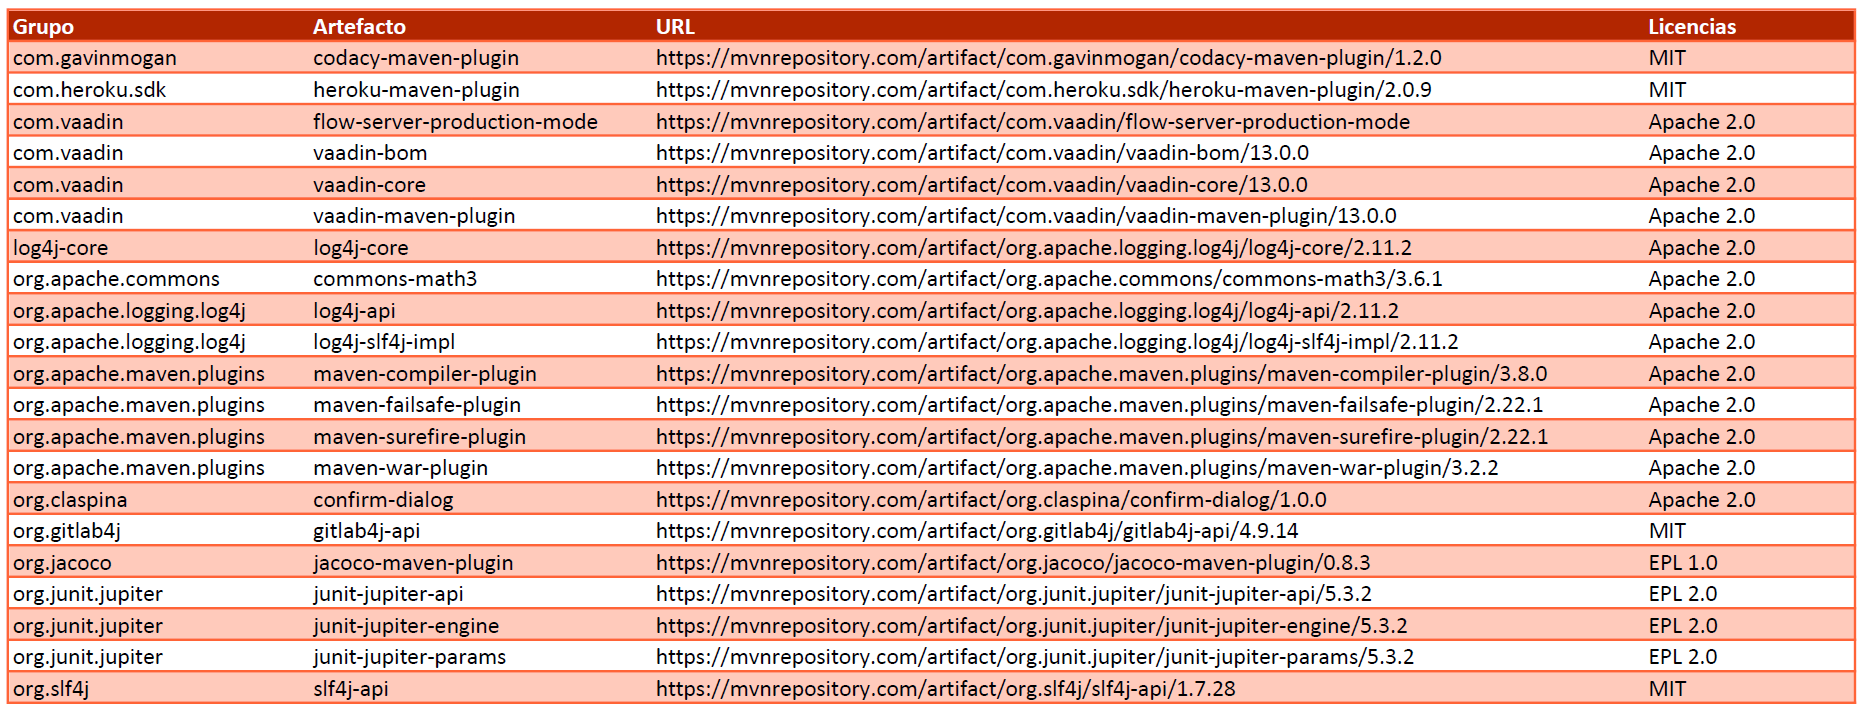
\includegraphics[scale=0.27]{AnexA_Licencias}
	\caption{Licencias de las dependencias del proyecto}
	\label{fig:AnexA_Licencias}
\end{figure}
\FloatBarrier

Por lo tanto, las licencias a las que está sometido nuestro proyecto son, de más a menos permisivas:
\begin{itemize}
	\item \textit{MIT}
	\item \textit{Apache v.2.0}
	\item \textit{EPL 2.0} --- La Fundación Eclipse informa que la versión 1.0 está en desuso y que los proyectos deben migrar a la versión 2.0, por lo tanto no nos restringe la versión 1.0 del plugin \textit{jacoco-maven-plugin}, sino la versión 2.0.
\end{itemize}

La licencia más restrictiva es la \textit{Eclipse Public License} que poseen las librerías que se utilizan para pruebas.

Nuestro proyecto puede tener la licencia \textit{GNU General Public License v3.0}, que permite el uso comercial, modificación, distribución, uso privado y el uso de patentes. Aunque no sea compatible, la nueva versión de \textit{EPL} permite utilizar la versión 2 de la \textit{GPL} de \textit{GNU} y posteriores como licencia secundaria en una parte especifica del código, eso garantiza la compatibilidad de ese código con esas versiones de la GPL \cite{santiago_lista_2019}. Por lo tanto, se puede licenciar el código bajo \textit{GPL v3.0} y el código de pruebas bajo licencia \textit{EPL} o compatibles como \textit{Apache v2.0}.